\documentclass[14pt,a4paper,oneside]{report}

\usepackage{pdfpages}
\usepackage{epstopdf}
\usepackage{url}
\usepackage{listings}
\usepackage{subfig}


\renewcommand{\thesection}{\arabic{section}}
\setcounter{secnumdepth}{3}

\title{\textbf{Optimal decision making for complex problems}
\\ Lunar Lander}

\author{Francois Delarbre \and Simon Lorent}


\begin{document}

\vfill
\date{Academic year 2017 - 2018}

\maketitle

\section{Introduction}
\paragraph{} In this project, we have chose to try to solve the lunar lander\footnote{\url{https://gym.openai.com/envs/LunarLander-v2/}} probleme from openAi gym. To do so, we have tryied two methods, the first one, by adapting code found\footnote{\url{https://www.superdatascience.com/artificial-intelligence/}} for an other problem, which use deep convolutional Q-learning. For the second one we tryied 
	to implement A3C algorithm by ourself. 
	
\section{A3C algorithm}
We have tried to implement the Asynchronous Advantage Actor-Critic introduced by 
Google DeepMind Group. 
This algorithm is a evolution of Deep Convolutonal Q-learning algorithm. It 
uses multiple asynchronous agents that iterract with the environement to get 
multiple experience that are independent from each other.  It also combine 
the main advantages of policy gradient and Q-learning in a single algorithm.
We wanted to implemente this method because it is one of the state of art one 
in reinforment learning.
We fisrt adapted to our problem a open-source code available on github 
\footnote{\url{https://github.com/awjuliani/DeepRL-Agents/blob/master/A3C-Doom.ipynb}}.
Unfortunately, we didn't manage to have a working version with our 
environement because of some multi-threading issues. As the error came from the 
graphic of the lunar lander environement  and the time was missing, we choosed to 
implement a algorithlm that doesn't require complex multi-threading.


\section{Deep Convolutional Q-learning}
\paragraph{} Deep convolutional Q-learning, as the name says, make use of a convolutional neural network, which take as an input images of the problem, and output the Q value for each actions. 
\subsection{Eligibility trace}
\paragraph{} The eligibiltiy trace consist of taking in account more of the pasts reward than the normal Q-learning. In traditional Q-learning, one compute the temporal difference as $TD = r_{k+1} + \gamma max\hat{Q}(x_{k+1}, u) − \hat{Q}(x_k, u_k)$. In the case of Eligibility Trace, one use $$TD^{(n)} = r_{k+1} + \gamma r_{k+1} + \gamma^2  r_{k+2} + ... + \gamma^{n-1}  r_{k+n-1} + \gamma^n max\hat{Q}(x_{k+1}, u) − \hat{Q}(x_k, u_k)$$

This allow to take more in account what happend in the past. Thus, the neural network uses the predicted Q values by it output and the computed one to compute the mean squared error loss  to update its weights. 

\subsection{Experience replay}
\paragraph{} For each action taken, the algorithm push to a buffer, this allows to have the benefits of experience replay, by sampling this buffer in order to train the neural network. 
\subsection{Performances}
\paragraph{} After a few epochs, the average reward on the last 100 steps is increasing, and it seems that it has understood that it has to land between the flags, but it seems that it takes longer to understand how to manoeuvring to land there. 

As we can see at \textbf{ figure \ref{fig1}}, the score is pretty low at the begining and then slowly increase. We can see a peak in the first epochs, this by luck, indeed, when exploring, it might encounter "good" states randomly. Running the program again would give different score. 
\begin{figure}
	\centering
	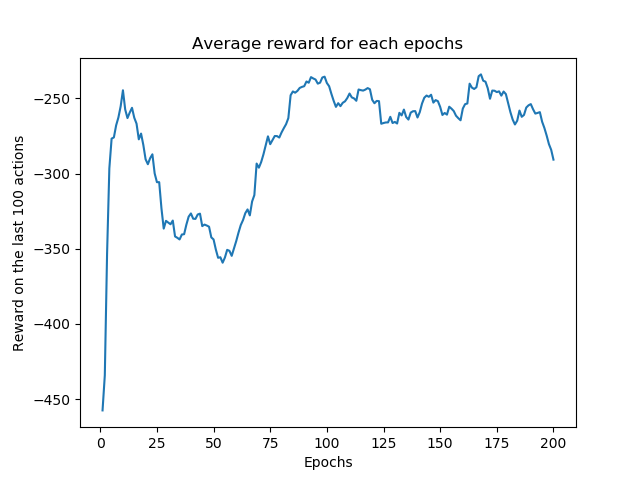
\includegraphics[width=\textwidth]{Figure_1.png}
	\caption{}
	\label{fig1}
\end{figure}

\paragraph{} In order to improve the performance, there is two way to search, the first one simply consist in running the training for a higher number of epochs, the second one consist of reviewing the convolutional neural network architecture and might lead to better results. 
\appendix
\chapter{Installation}
\section{Needed components}
\paragraph{} In order to run the code, it is needed to install first openAI gym lunar lander v2 environement, then tensorflow is needed for the A3C part, the deep convolutional Q-learning requiere pytorch, cuda version to be installed. And thus it need a working version of cuda installed on a linux machine. 



\end{document}
